% fig_tr_timeline.tex
% TR-28: Horizontal research arc timeline for SAMBP TR-03 through TR-27
%
% Four arcs:
%   Arc 1 (blue):   TR-03--04   Core model-based framework
%   Arc 2 (green):  TR-05--11   System validation
%   Arc 3 (orange): TR-12--19   87L line differential enhancements
%   Arc 4 (purple): TR-20--27   IBR protection chain
%
% Layout: each TR is a node on a horizontal axis; arc boundaries shown
% with coloured braces; key results annotated below milestone TRs.

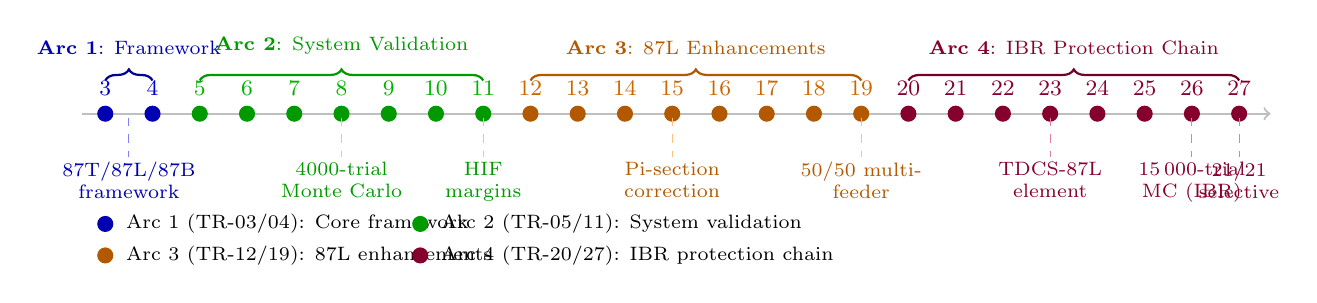
\begin{tikzpicture}[
  every node/.style={font=\scriptsize},
  trnode/.style={circle, minimum size=5pt, inner sep=0pt, draw, thick},
  arc1/.style={fill=blue!70!black, draw=blue!70!black},
  arc2/.style={fill=green!60!black, draw=green!60!black},
  arc3/.style={fill=orange!70!black, draw=orange!70!black},
  arc4/.style={fill=purple!70!black, draw=purple!70!black},
]

% ---- Horizontal axis line ----
\draw[->,gray!50, thick] (-0.3,0) -- (14.8,0);

% ---- TR positions: TRs 3-27, spaced 0.6 apart starting at x=0 ----
% x = (TR# - 3) * 0.6
% TR3=0, TR4=0.6, TR5=1.2, TR6=1.8, TR7=2.4, TR8=3.0,
% TR9=3.6, TR10=4.2, TR11=4.8, TR12=5.4, TR13=6.0,
% TR14=6.6, TR15=7.2, TR16=7.8, TR17=8.4, TR18=9.0,
% TR19=9.6, TR20=10.2, TR21=10.8, TR22=11.4, TR23=12.0,
% TR24=12.6, TR25=13.2, TR26=13.8, TR27=14.4

% ---- Arc 1: TR-03, TR-04 ----
\foreach \tr/\x in {3/0, 4/0.6} {
  \node[trnode, arc1] (n\tr) at (\x,0) {};
  \node[above=3pt, blue!80!black] at (\x,0) {\footnotesize \tr};
}
\draw[blue!60!black, thick, decorate, decoration={brace, amplitude=4pt, raise=12pt}]
  (0,0) -- (0.6,0);
\node[blue!70!black, above=18pt] at (0.3,0) {\textbf{Arc 1}: Framework};

% ---- Arc 2: TR-05 to TR-11 ----
\foreach \tr/\x in {5/1.2, 6/1.8, 7/2.4, 8/3.0, 9/3.6, 10/4.2, 11/4.8} {
  \node[trnode, arc2] (n\tr) at (\x,0) {};
  \node[above=3pt, green!70!black] at (\x,0) {\footnotesize \tr};
}
\draw[green!60!black, thick, decorate, decoration={brace, amplitude=4pt, raise=12pt}]
  (1.2,0) -- (4.8,0);
\node[green!60!black, above=18pt] at (3.0,0) {\textbf{Arc 2}: System Validation};

% ---- Arc 3: TR-12 to TR-19 ----
\foreach \tr/\x in {12/5.4, 13/6.0, 14/6.6, 15/7.2, 16/7.8, 17/8.4, 18/9.0, 19/9.6} {
  \node[trnode, arc3] (n\tr) at (\x,0) {};
  \node[above=3pt, orange!80!black] at (\x,0) {\footnotesize \tr};
}
\draw[orange!70!black, thick, decorate, decoration={brace, amplitude=4pt, raise=12pt}]
  (5.4,0) -- (9.6,0);
\node[orange!70!black, above=18pt] at (7.5,0) {\textbf{Arc 3}: 87L Enhancements};

% ---- Arc 4: TR-20 to TR-27 ----
\foreach \tr/\x in {20/10.2, 21/10.8, 22/11.4, 23/12.0, 24/12.6, 25/13.2, 26/13.8, 27/14.4} {
  \node[trnode, arc4] (n\tr) at (\x,0) {};
  \node[above=3pt, purple!70!black] at (\x,0) {\footnotesize \tr};
}
\draw[purple!60!black, thick, decorate, decoration={brace, amplitude=4pt, raise=12pt}]
  (10.2,0) -- (14.4,0);
\node[purple!70!black, above=18pt] at (12.3,0) {\textbf{Arc 4}: IBR Protection Chain};

% ---- Milestone annotations below axis ----
\draw[blue!50, dashed] (0.3,-0.05) -- (0.3,-0.55);
\node[blue!70!black, below=14pt, align=center] at (0.3,0)
  {87T/87L/87B\\framework};

\draw[green!50, dashed] (3.0,-0.05) -- (3.0,-0.55);
\node[green!60!black, below=14pt, align=center] at (3.0,0)
  {4000-trial\\Monte Carlo};

\draw[green!50, dashed] (4.8,-0.05) -- (4.8,-0.55);
\node[green!60!black, below=14pt, align=center] at (4.8,0)
  {HIF\\margins};

\draw[orange!50, dashed] (7.2,-0.05) -- (7.2,-0.55);
\node[orange!70!black, below=14pt, align=center] at (7.2,0)
  {Pi-section\\correction};

\draw[orange!50, dashed] (9.6,-0.05) -- (9.6,-0.55);
\node[orange!70!black, below=14pt, align=center] at (9.6,0)
  {50/50 multi-\\feeder};

\draw[purple!50, dashed] (12.0,-0.05) -- (12.0,-0.55);
\node[purple!70!black, below=14pt, align=center] at (12.0,0)
  {TDCS-87L\\element};

\draw[purple!50, dashed] (13.8,-0.05) -- (13.8,-0.55);
\node[purple!70!black, below=14pt, align=center] at (13.8,0)
  {15\,000-trial\\MC (IBR)};

\draw[purple!50, dashed] (14.4,-0.05) -- (14.4,-0.55);
\node[purple!70!black, below=14pt, align=center] at (14.4,0)
  {21/21\\selective};

% ---- Legend ----
\node[arc1, trnode] at (0,-1.4) {};
\node[right=4pt] at (0,-1.4) {Arc 1 (TR-03/04): Core framework};
\node[arc2, trnode] at (4,-1.4) {};
\node[right=4pt] at (4,-1.4) {Arc 2 (TR-05/11): System validation};
\node[arc3, trnode] at (0,-1.8) {};
\node[right=4pt] at (0,-1.8) {Arc 3 (TR-12/19): 87L enhancements};
\node[arc4, trnode] at (4,-1.8) {};
\node[right=4pt] at (4,-1.8) {Arc 4 (TR-20/27): IBR protection chain};

\end{tikzpicture}
